\section{Simulation Details}
\label{sec:simulation}

In order to study jet images in a realistic scenario, we use Monte Carlo (MC) simulations of high energy particle collisions. One important jet tagging application is the identification of highly Lorentz boosted $W$ bosons decaying into quarks amidst a large background from the generic production of quarks and gluons.  This classification task has been thoroughly studied experimentally\footnote{There is also an extensive literature on phenomenological studies - see references within the experimental papers.}~\cite{Khachatryan:2014vla,ATL-PHYS-PUB-2015-033,ATL-PHYS-PUB-2014-004} and used in many experimental analyses~\cite{Aad:2015owa,Khachatryan:2014hpa,Khachatryan:2015mta,Khachatryan:2015oba,Khachatryan:2015gza,Khachatryan:2015bma,Khachatryan:2015cwa,Khachatryan:2015ywa,Aad:2014wea,Aad:2015agg,Aad:2015kna,Aad:2015ufa,Aad:2014haa}.  

To simulate highly boosted $W$ bosons, a hypothetical $W'$ boson is generated and forced to decay to a hadronically decaying $W$ boson ($W\rightarrow qq'$) and a $Z$ boson which decays invisibly ($Z\rightarrow \nu\bar{\nu}$).  The mass of the $W'$ boson determines the Lorentz boost of the $W$ boson in the lab frame since the $W'$ is produced nearly at rest and the $W$ boson momentum is approximately $m_{W'}/2$.  Multijet production of quarks and gluons is simulated as a background.  Both the $W'$ signal and the multijet background are generated using \textsc{Pythia} 8.170~\cite{Pythia8,Pythia} at $\sqrt{s}=14$ TeV.  The angular separation of the $W$ boson decay products in the plane transverse to the beam direction scales as $2m_{W}/p_{T,W}$, where $m_W\approx 80$~GeV and $p_{T,W}$ is the component of the $W$ boson momentum in this plane.  The tagging strategy and performance depend strongly on $p_{T,W}$, so we focus on a particular range: $250$~GeV~$<p_{T,W}<300$~GeV.  This corresponds to an angular spread of about $1$ radian.  The decay products of the $W$ bosons as well as the background are clustered into jets using the anti-$k_t$ algorithm~\cite{antiktpaper} via \textsc{FastJet}~\cite{fastjet} 3.0.3.  To mitigate the contribution from the underlying event, jets are are trimmed~\cite{trimming} by re-clustering the constituents into $R=0.3$ $k_t$ subjets and dropping those which have $p_T^\text{subjet}<0.05\times p_T^\text{jet}$. 

To model the discretization and finite acceptance of a real detector, a calorimeter of towers with size $0.1\times 0.1$ in $(y,\phi)$ extends out to $y=5.0$.  The total energy of the simulated particles incident upon a particular cell are added as scalars and the four-vector $p_j$ of any particular tower $j$ is given by

\begin{align}
\label{eq:calo}
p_j = \sum_{i\text{ incident on $j$}}E_i(\cos\phi_j/\cosh y_j,\sin\phi_j/\cosh y_j,\sinh y_j/\cosh y_j,1).
\end{align}


\begin{figure}[bt]
  \begin{center}
      \subfloat[Unweighted $p_T$ distribution \label{subfig:unweighted_pt}]{
        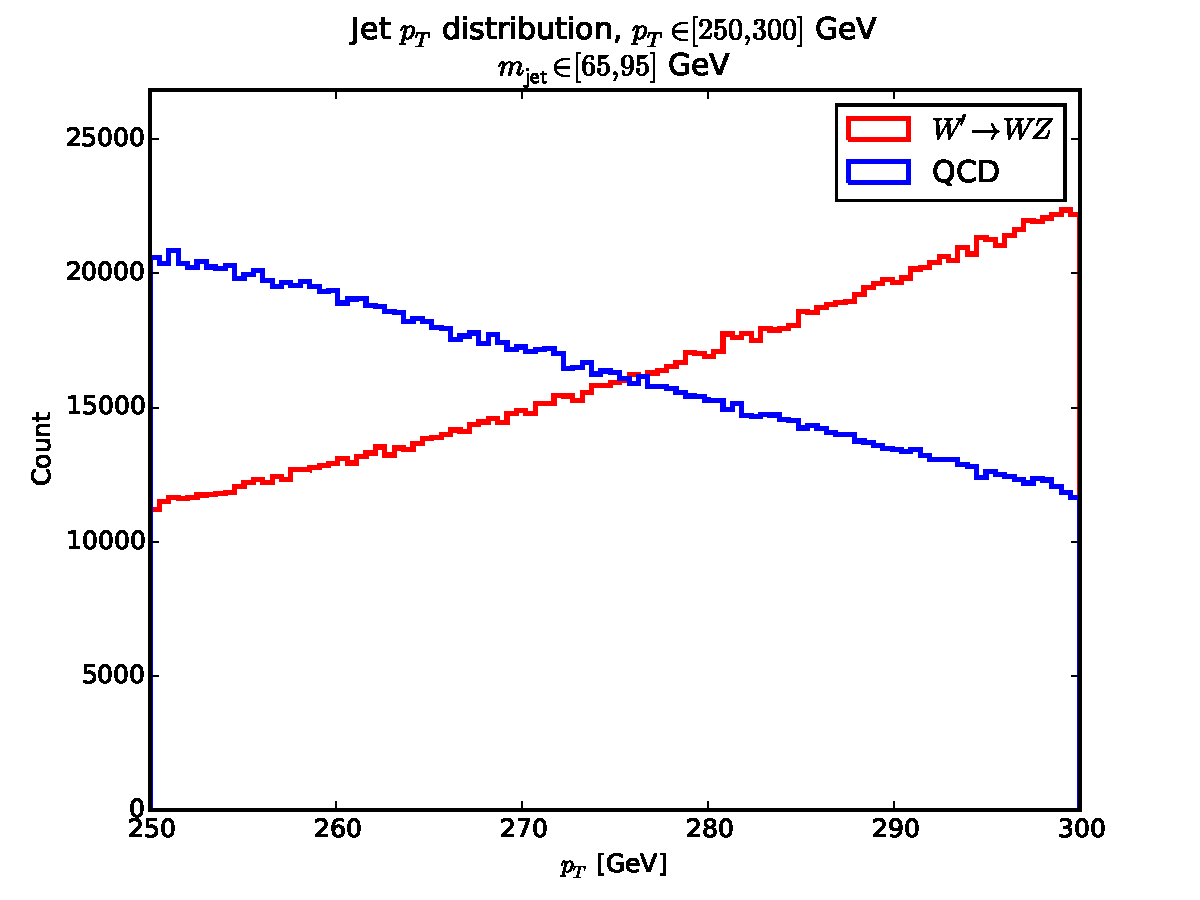
\includegraphics[width=0.5\textwidth]{figures/unweighted-pt-distribution-[250-300].pdf}
      }
      \subfloat[Weighted $p_T$ distribution \label{subfig:weighted_pt}]{
        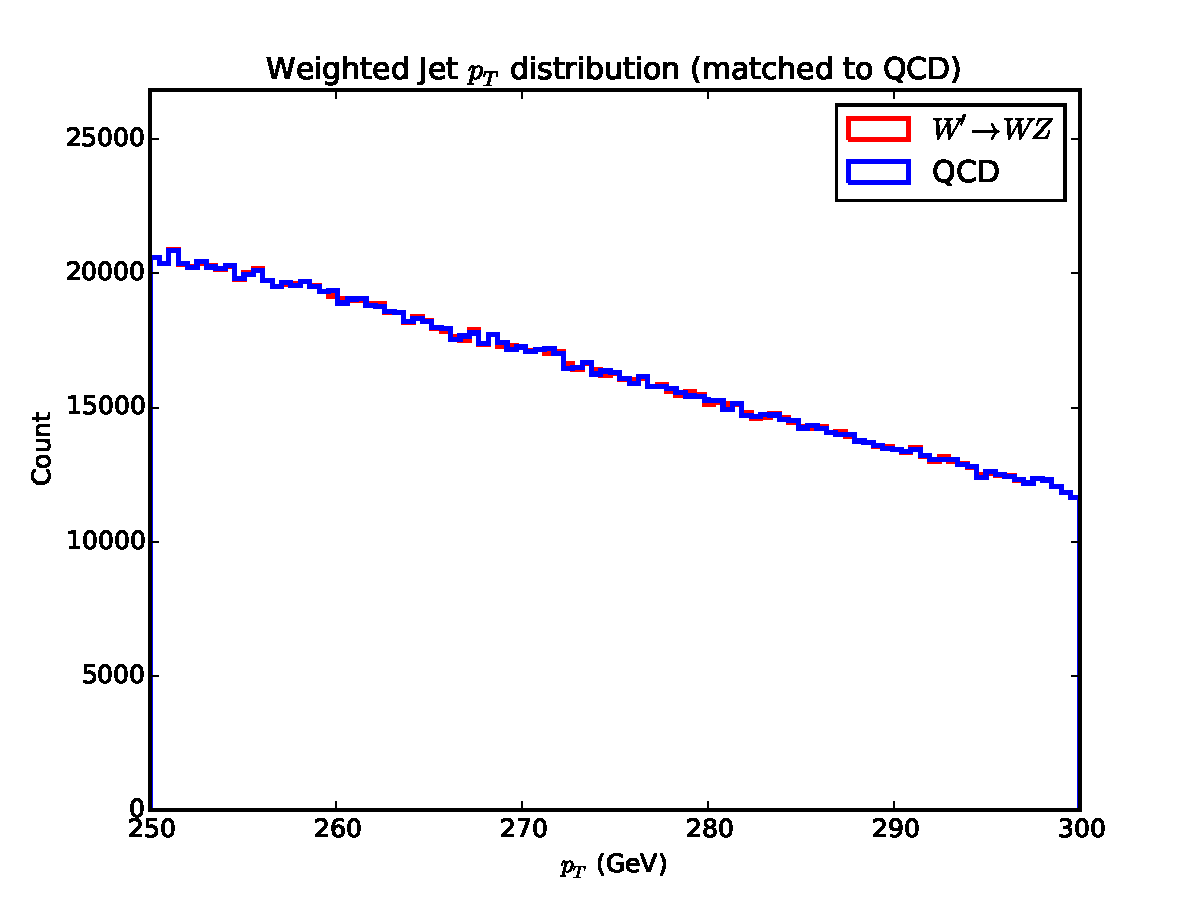
\includegraphics[width=0.5\textwidth]{figures/weighted-pt-distribution[250-300].pdf}
      }
      \caption{ Jets originating from the $W'\rightarrow WZ$ decay are re-weighted such that their $p_T$ spectrum matches that of QCD jets\label{fig:pt} }
    \end{center}
\end{figure}


\begin{figure}[bt]
  \begin{center}
  
  
      \subfloat[Weighted jet mass distribution \label{subfig:weighted_mass}]{
        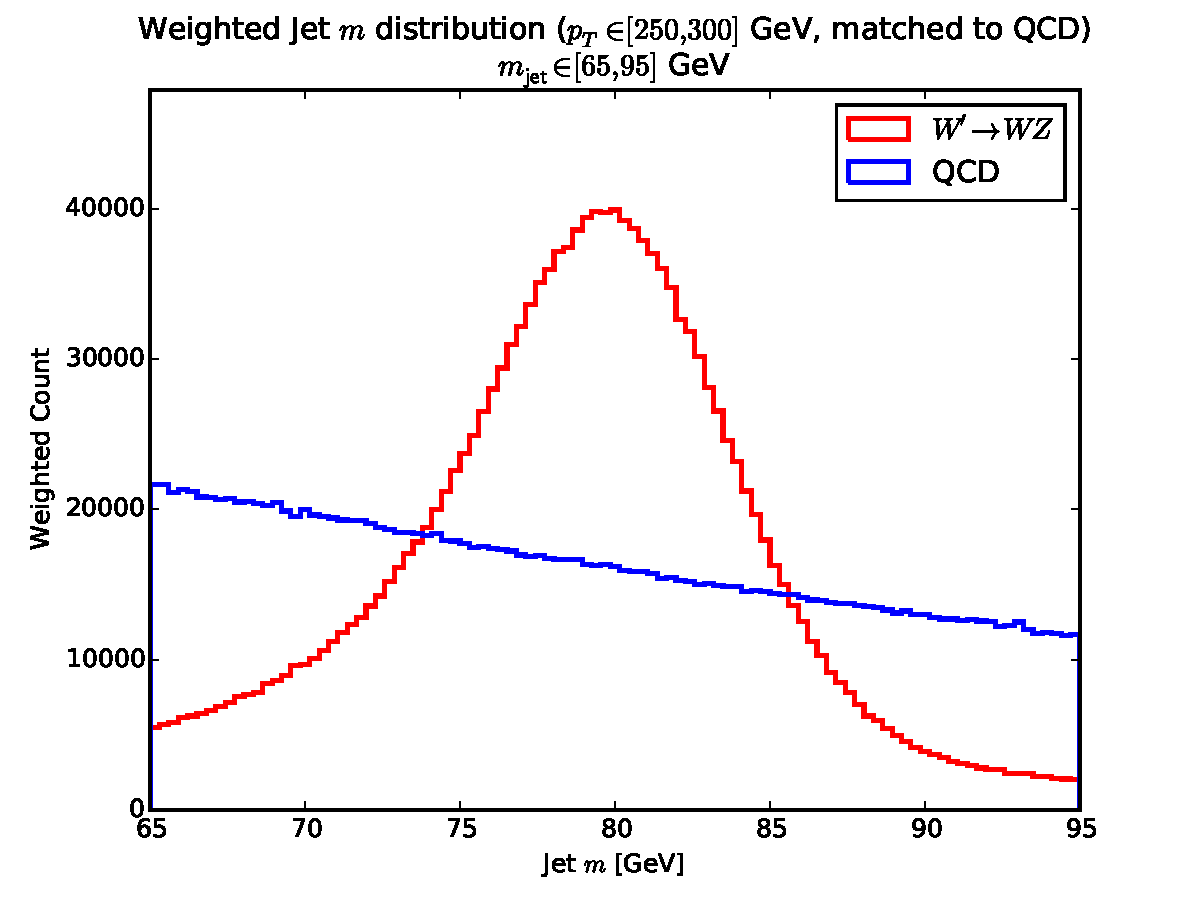
\includegraphics[width=0.5\textwidth]{figures/weighted-mass-distribution[250-300].pdf}
      }
      \subfloat[Weighted $\tau_{21}$ distribution \label{subfig:weighted_nsj}]{
        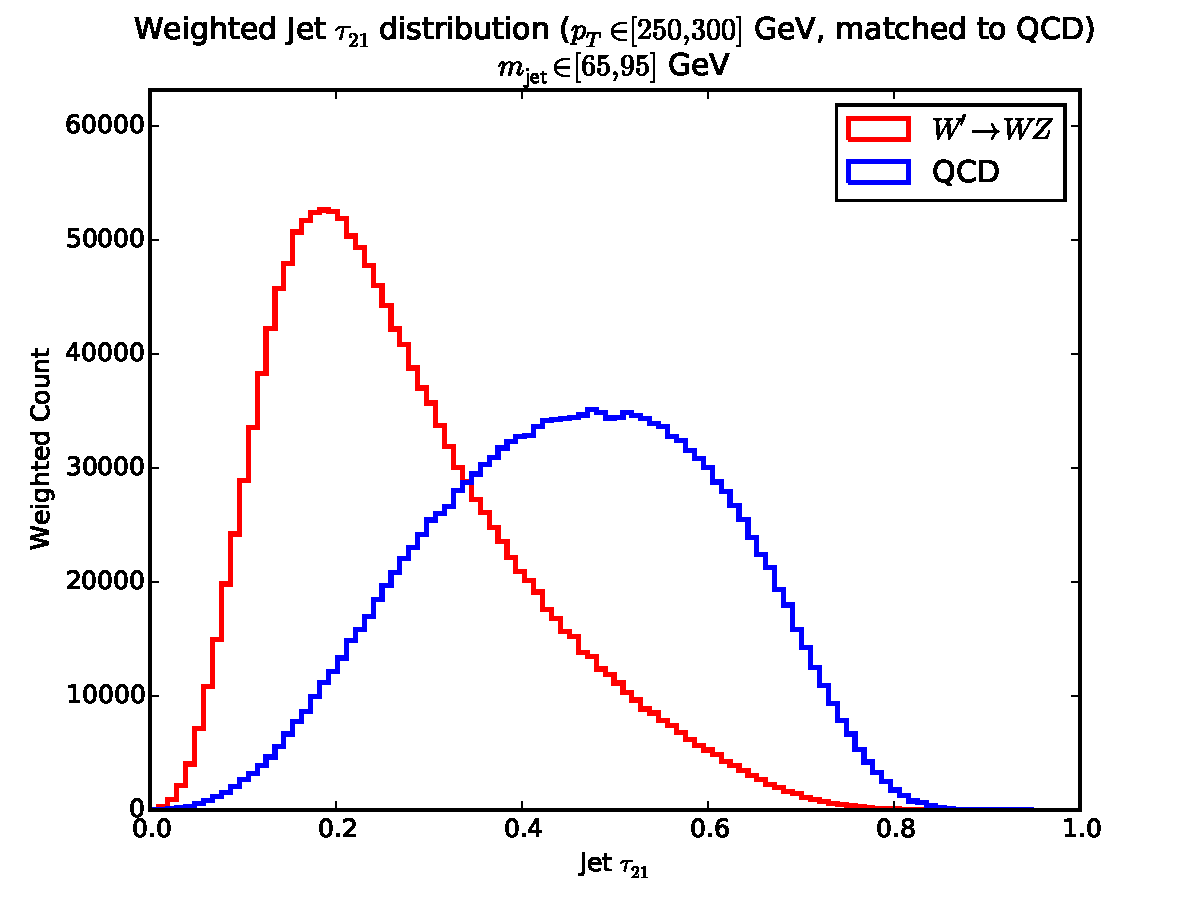
\includegraphics[width=0.5\textwidth]{figures/weighted-tau21-distribution[250-300].pdf}
      }
      \caption{Weighted mass (left) and $n$-subjettiness (right) of samples, with $W'\rightarrow WZ$ decays in red and QCD jets in blue.\label{fig:mass_nsj_spectrum} }
    \end{center}
\end{figure}  



\begin{figure}[bt]
  \begin{center}
  
      \subfloat[Average weighted $W'\rightarrow WZ$ image \label{subfig:weighted_sig}]{
        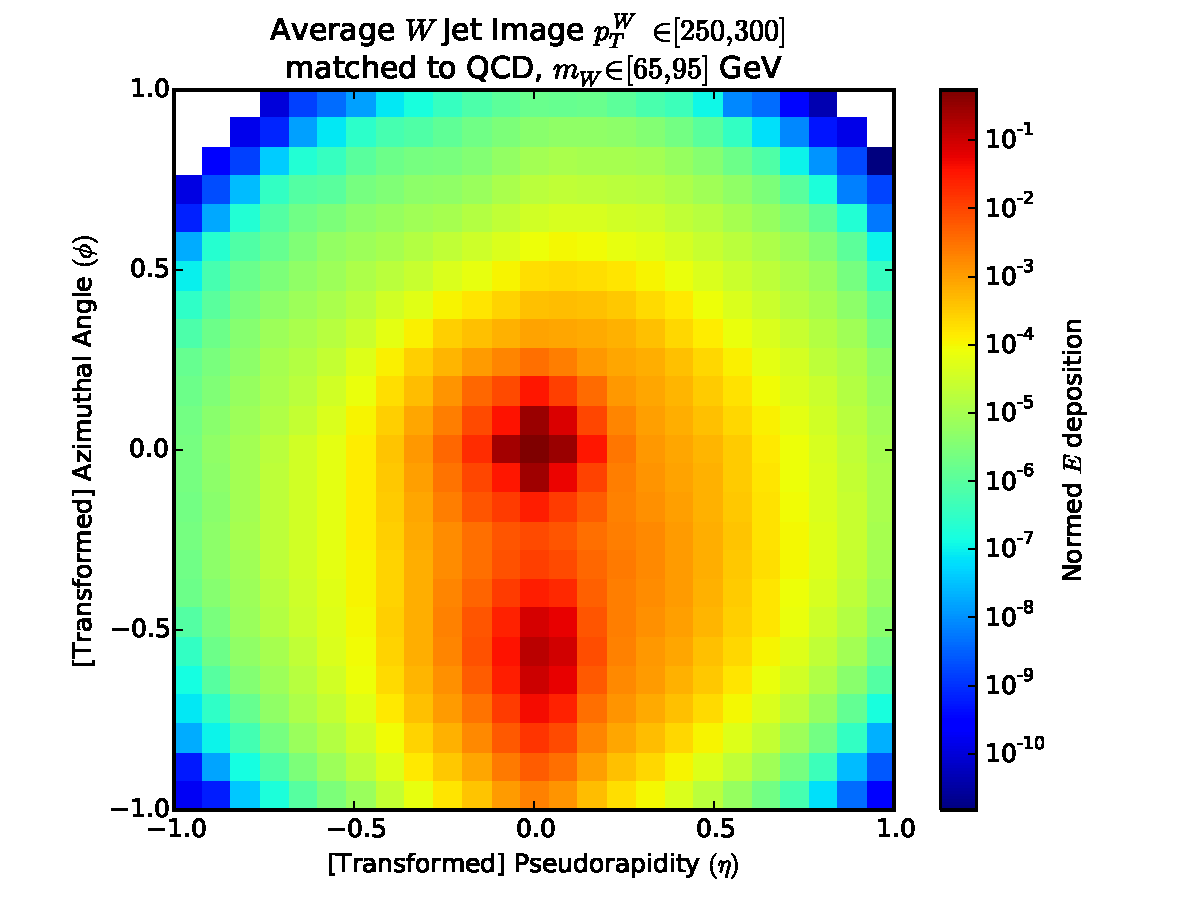
\includegraphics[width=0.5\textwidth]{figures/sig-im.pdf}
      }
      \subfloat[Average weighted QCD image \label{subfig:weighted_bkg}]{
        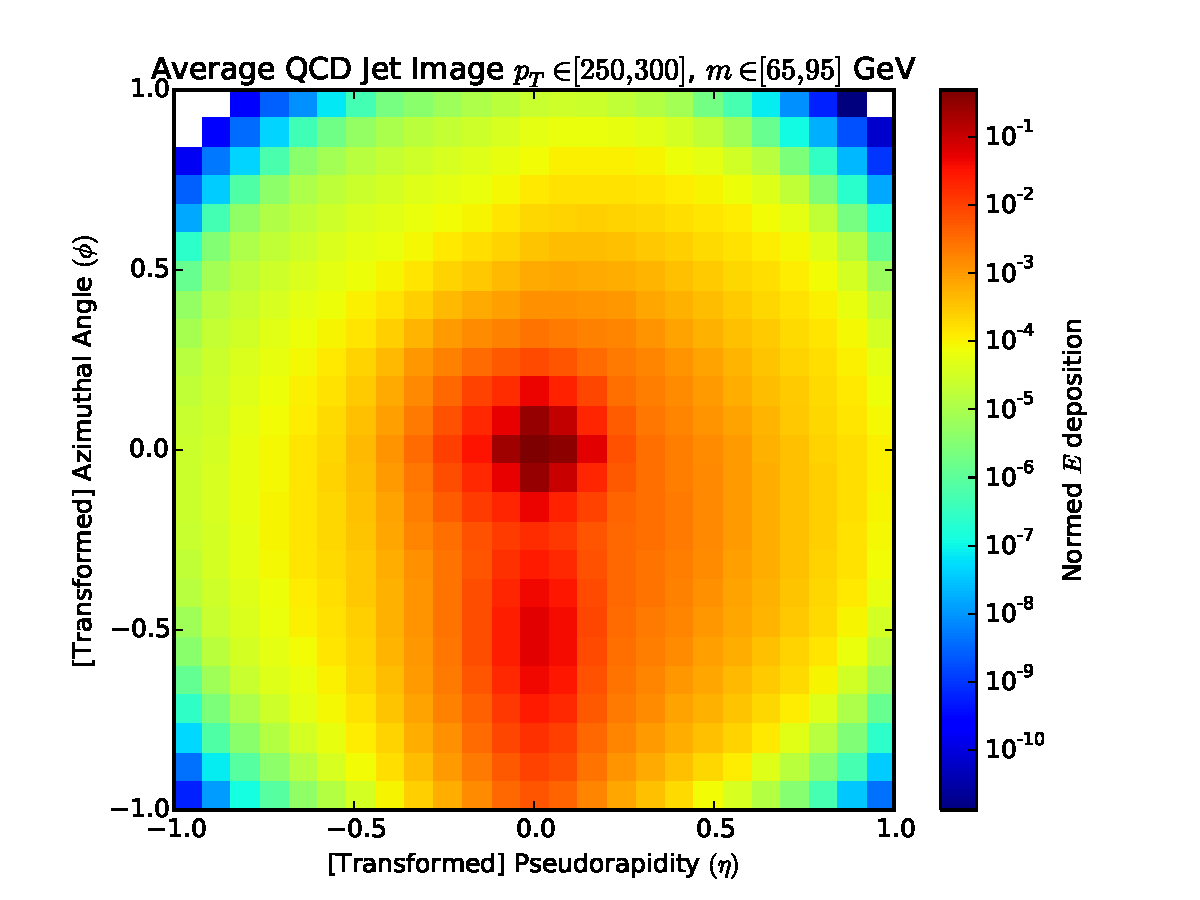
\includegraphics[width=0.5\textwidth]{figures/bkg-im.pdf}
      }
      \caption{Weighted $W'\rightarrow WZ$ (left) and QCD (right) average jet-image
      \label{fig:meanImages} }
    \end{center}
\end{figure}  

Discuss the creation of the jet images.

Discuss the physical differences between W bosons and q/g jets?
